\section{Red p'ublica}
Situados en un patio de comidas, monitoreamos la red wifi de un shopping importante durante 30 minutos con el objetivo de analizar una red
con muy poco control y en constante cambio.

El primer experimento, el cual ve la red como una fuente con 2 simbolos unicamente, resulto en n'umeros similares a la red hogare\~na 
aunque en un principio se podria suponer que el trafico broadcast iba a ser mucho mas elevado con tantos nodos entrando y saliendo
de la red. 

\begin{figure}[!h]
\centering
\caption{Informaci'on de S p'ublica}
\begin{tabular}{ r|c|c| }
\multicolumn{1}{r}{}
 &  \multicolumn{1}{c}{frecuencia}
 & \multicolumn{1}{c}{informaci'on} \\
\cline{2-3}
$S_{broadcast}$ & 0.21 & 2.25 \\
\cline{2-3}
$S_{unicast}$ & 0.79 & 0.34 \\
\cline{2-3}
\end{tabular}
\end{figure}
 
Estos valores nos dan una entrop'ia de 0.65 bits (siendo el m'aximo 1 dado que hay 2 simbolos en principio equiprobables). Suponemos
que la similitud con la red hogare\~na esta en que el tiempo en que monitoreamos la red coincide o es menor que el tiempo de cada nodo en la
red.
 
En el segundo experimento, el cual modela la red basado en la direcci'on a resolver en mensajes ARP, usamos la misma captura
utilizada en el experimento anterior. Nuestra herramienta y definici'on de nodo destacado encontr'o 2 nodos para destacar, uno sabemos que es
gateway por default mas no sabemos exactamente que es el segundo, posiblemente otro gateway para otro sector o diferentes clientes (dado
que analizando la direcci'on de enlace podemos ver que es un router de reconocida marca)
 
\begin{figure}[!h]
\centering
\caption{Informaci'on red p'ublica}
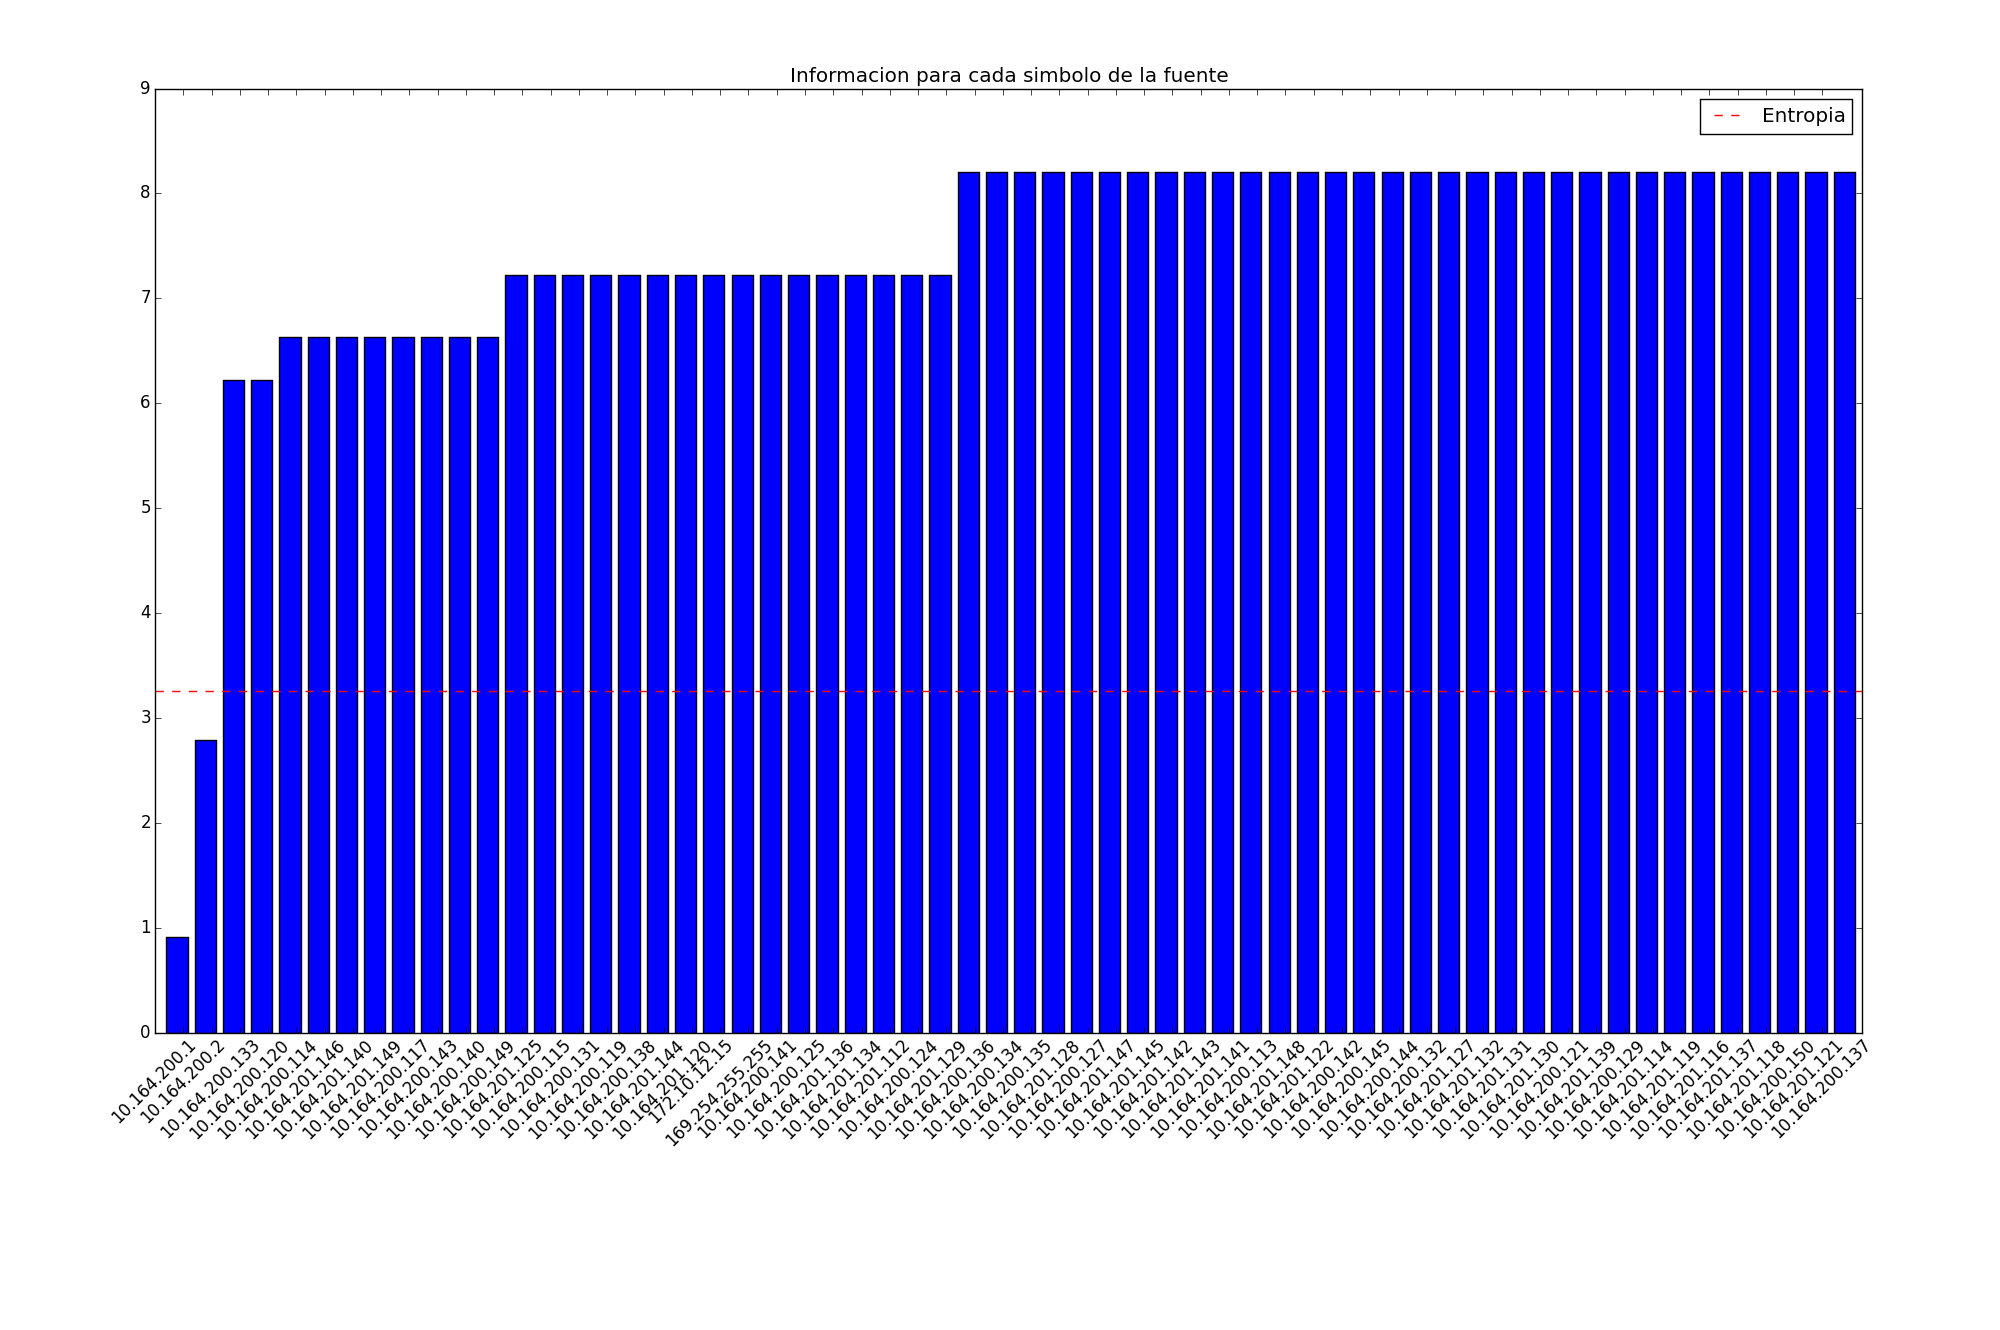
\includegraphics[width=0.75\textwidth]{red3_info}
 \label{fig:red3info}
\end{figure}

Se pueden notar 3 grupos de nodos basados en la informaci'on: destacados, aquellos que fueron accedidos dentro de la red por otros nodos y una
gran cola de nodos que solo figuran por un otro ARP capturado. Lo mismo se refleja en la visualizaci'on de la red a partir de la fuente S1
donde se puede ver como los nodos destacados son varias magnitudes m'as grandes que el resto. 

\begin{figure}[!h]
\caption{Visualizaci'on red p'ublica, en amarillo los nodos destacados}
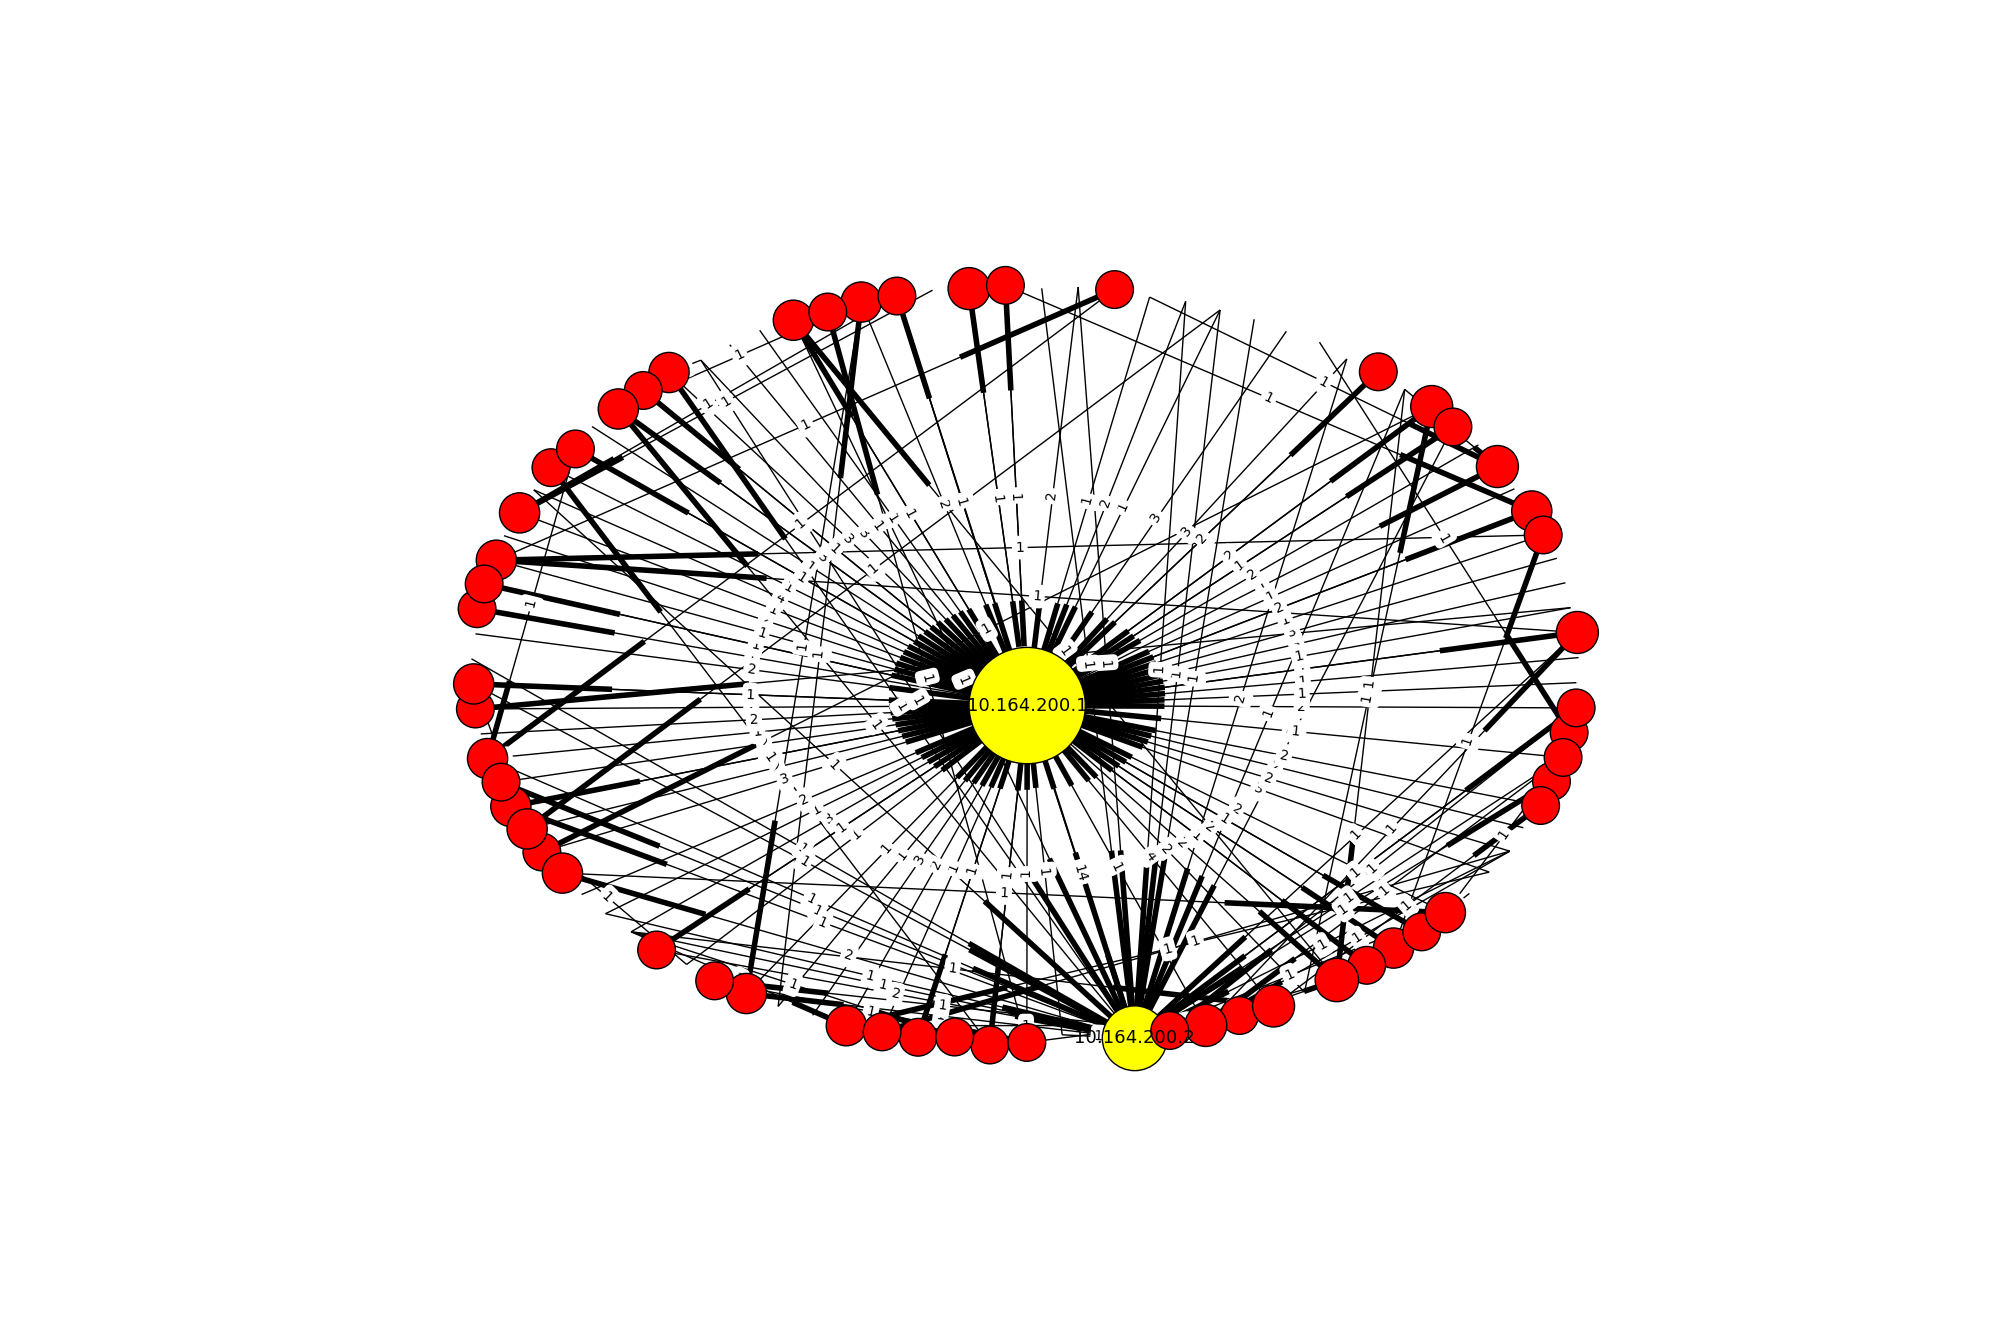
\includegraphics[width=1.1\textwidth]{red3_red}
 \label{fig:red3net}
\end{figure}

Al igual que la red laboral antes descripta volvimos a observar ARP gratuitos y ARP de sondeo provenientes del gateway y de algunos nodos.
